\documentclass[12pt]{beamer}
\mode<presentation> {
\usetheme{Madrid}
\setbeamertemplate{navigation symbols}{}
}

\usepackage{graphicx}
\usepackage{booktabs} % toprule, \midrule and \bottomrule in tables
\newcommand\hmmax{0}  % stop the 'too many math scripts' error
\newcommand\bmmax{0}
\usepackage{amsmath, amssymb, amsthm}  % advanced maths commands
\usepackage{float}  % bunch of formatting stuff
\usepackage{hyperref}
\usepackage{mathtools}
\usepackage{siunitx}
\usepackage[center]{caption}


%TITLE PAGE
\title[Blob-match]{Blob-match: Machine learning for cross-identification of radio surveys}

\author[James Gardner]{James Gardner, supervisors:\ Cheng Soon Ong, Matthew Alger}
\date{October 22, 2019}

\begin{document}

\begin{frame}
\titlepage
\end{frame}

\begin{frame}{What's out there in the universe?}
\begin{figure}
    \centering
    \scalebox{-1}[1]{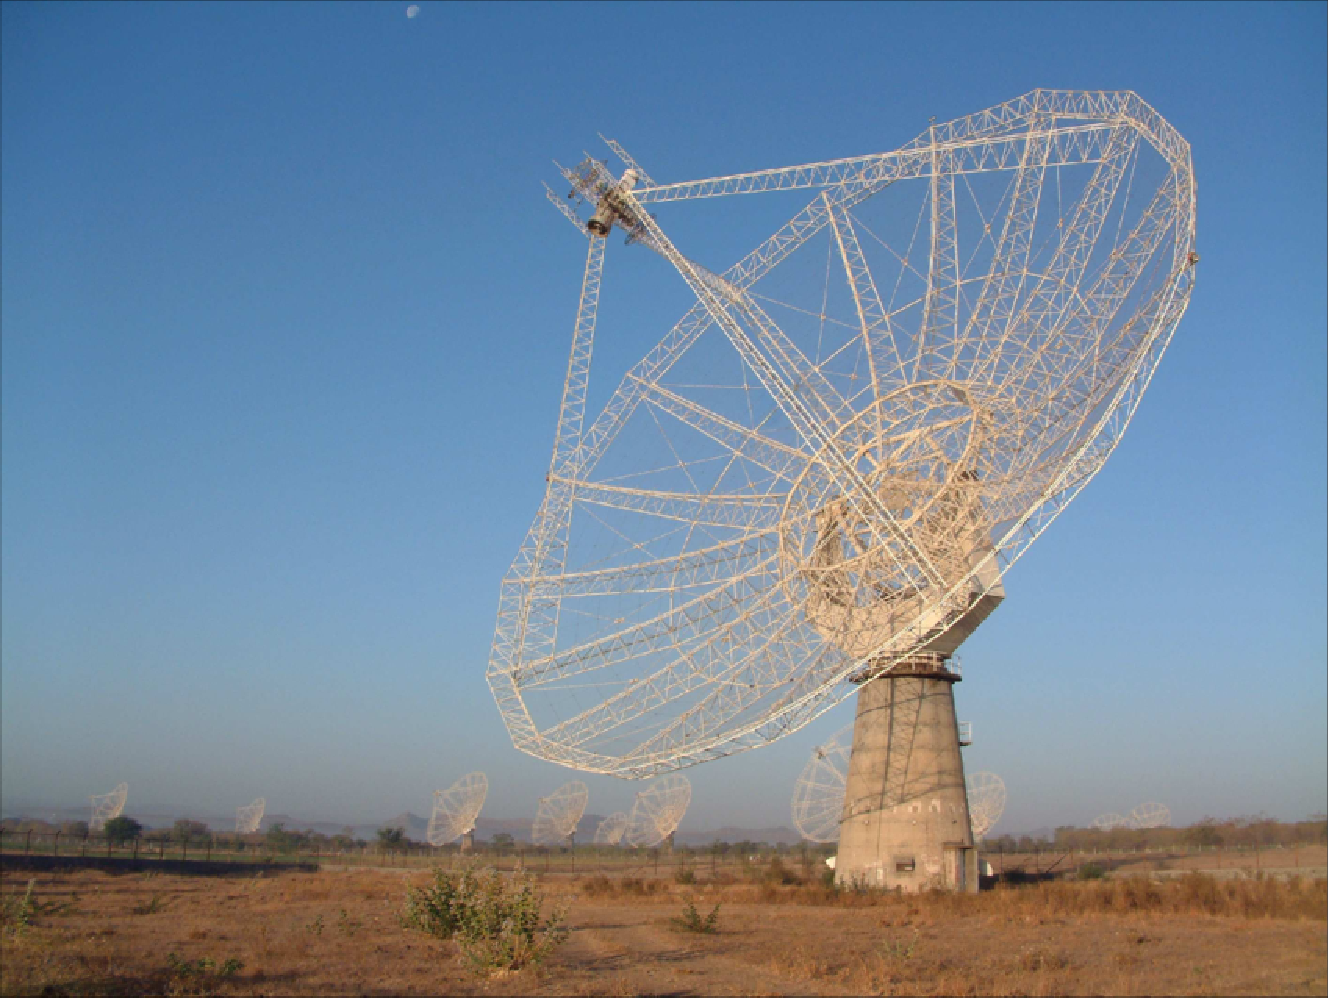
\includegraphics[width=0.44\textwidth]{pics/GMRT.pdf}} \;\;
    \scalebox{-1}[1]{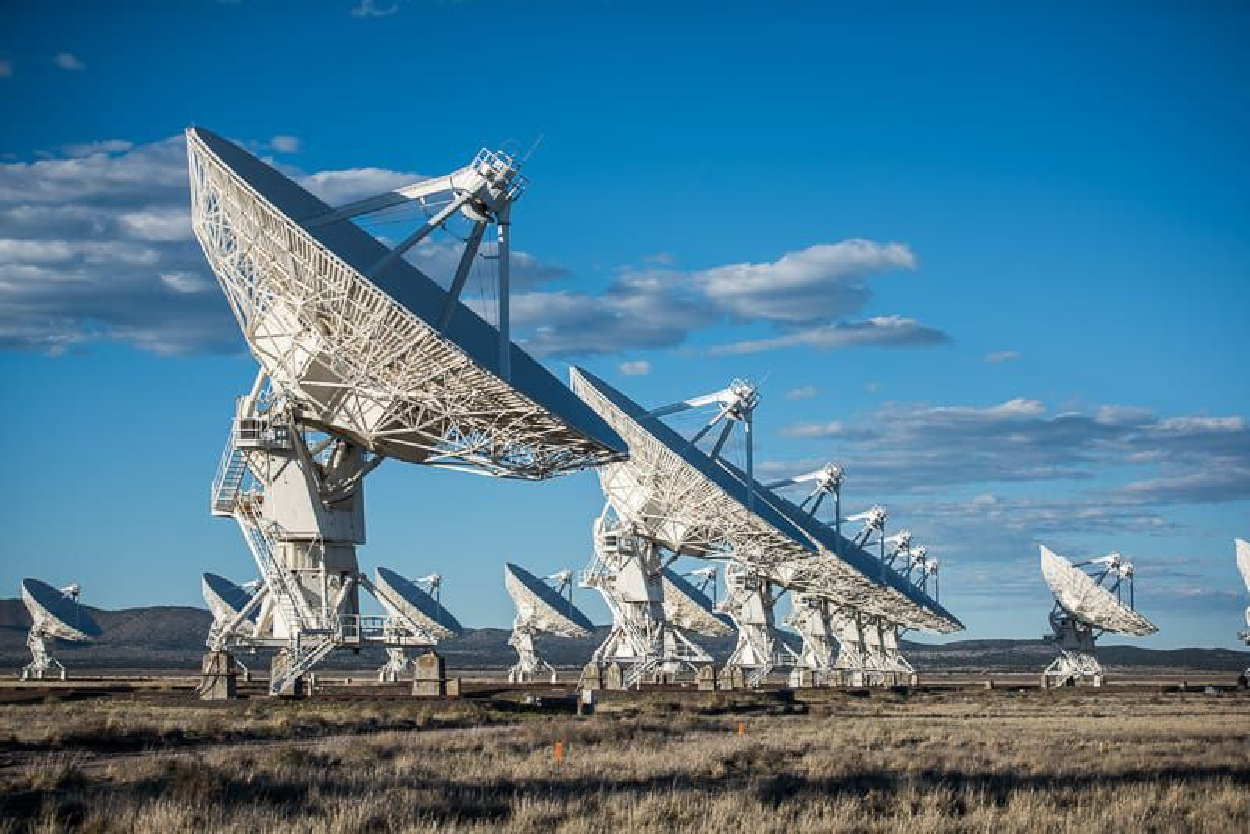
\includegraphics[width=0.5\textwidth]{pics/VLA.pdf}}
    \caption{Giant Metrewave Radio Telecope and Very Large Array\\
    (TGSS) 150 MHz / resolution $\ang{;;25}$ vs. (NVSS) 1.4 GHz / resolution $\ang{;;45}$}
\end{figure}
\end{frame}

\begin{frame}{Cross-identification}
\begin{figure}
    \centering
    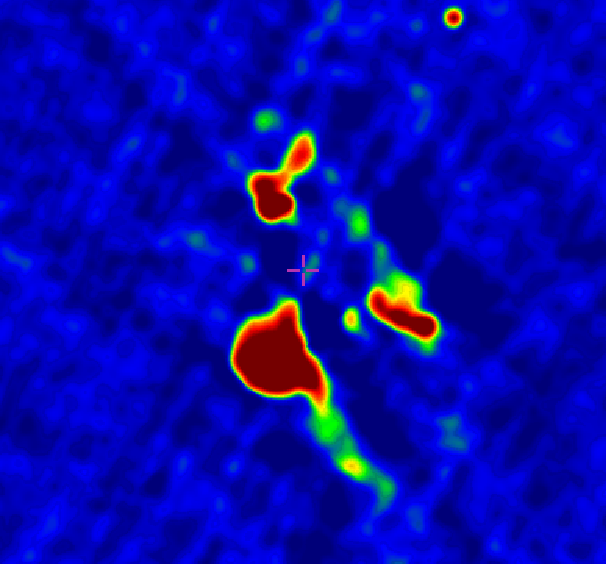
\includegraphics[width=0.48\textwidth]{pics/3c40t-cropped.pdf} \;\;
    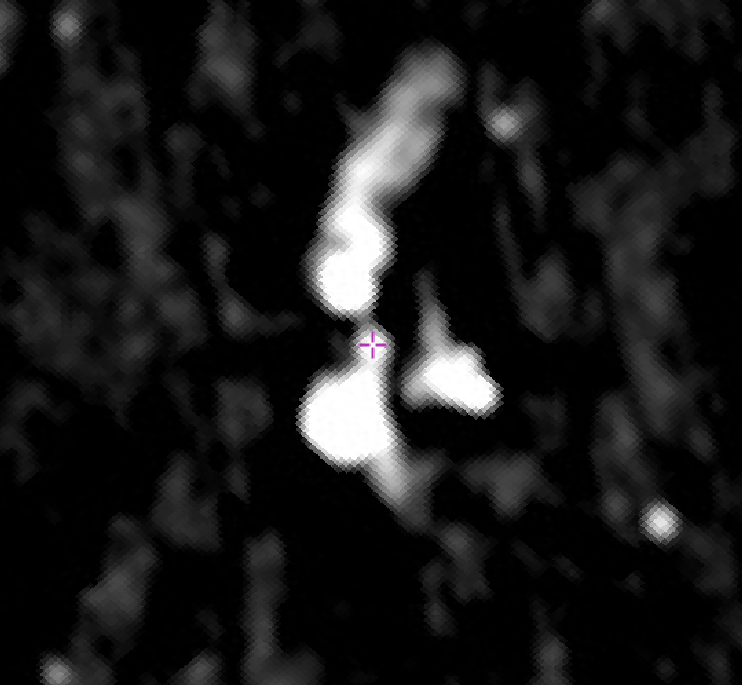
\includegraphics[width=0.48\textwidth]{pics/3c40n-cropped.pdf}
    \caption{Sources (blobs) of 3c40 in TGSS and NVSS}
\end{figure}
\end{frame}

% preview of coming attractions
\begin{frame}{Conclusions to come}
\begin{block}{Reproduction of existing positional matching results}
\end{block}
\begin{exampleblock}{Success of classifier trained on positional matching}
\end{exampleblock}
\begin{alertblock}{Failure of naive transitive partitioning}
\end{alertblock}
\end{frame}

\begin{frame}{Positional matching}
\begin{figure}
    \centering
    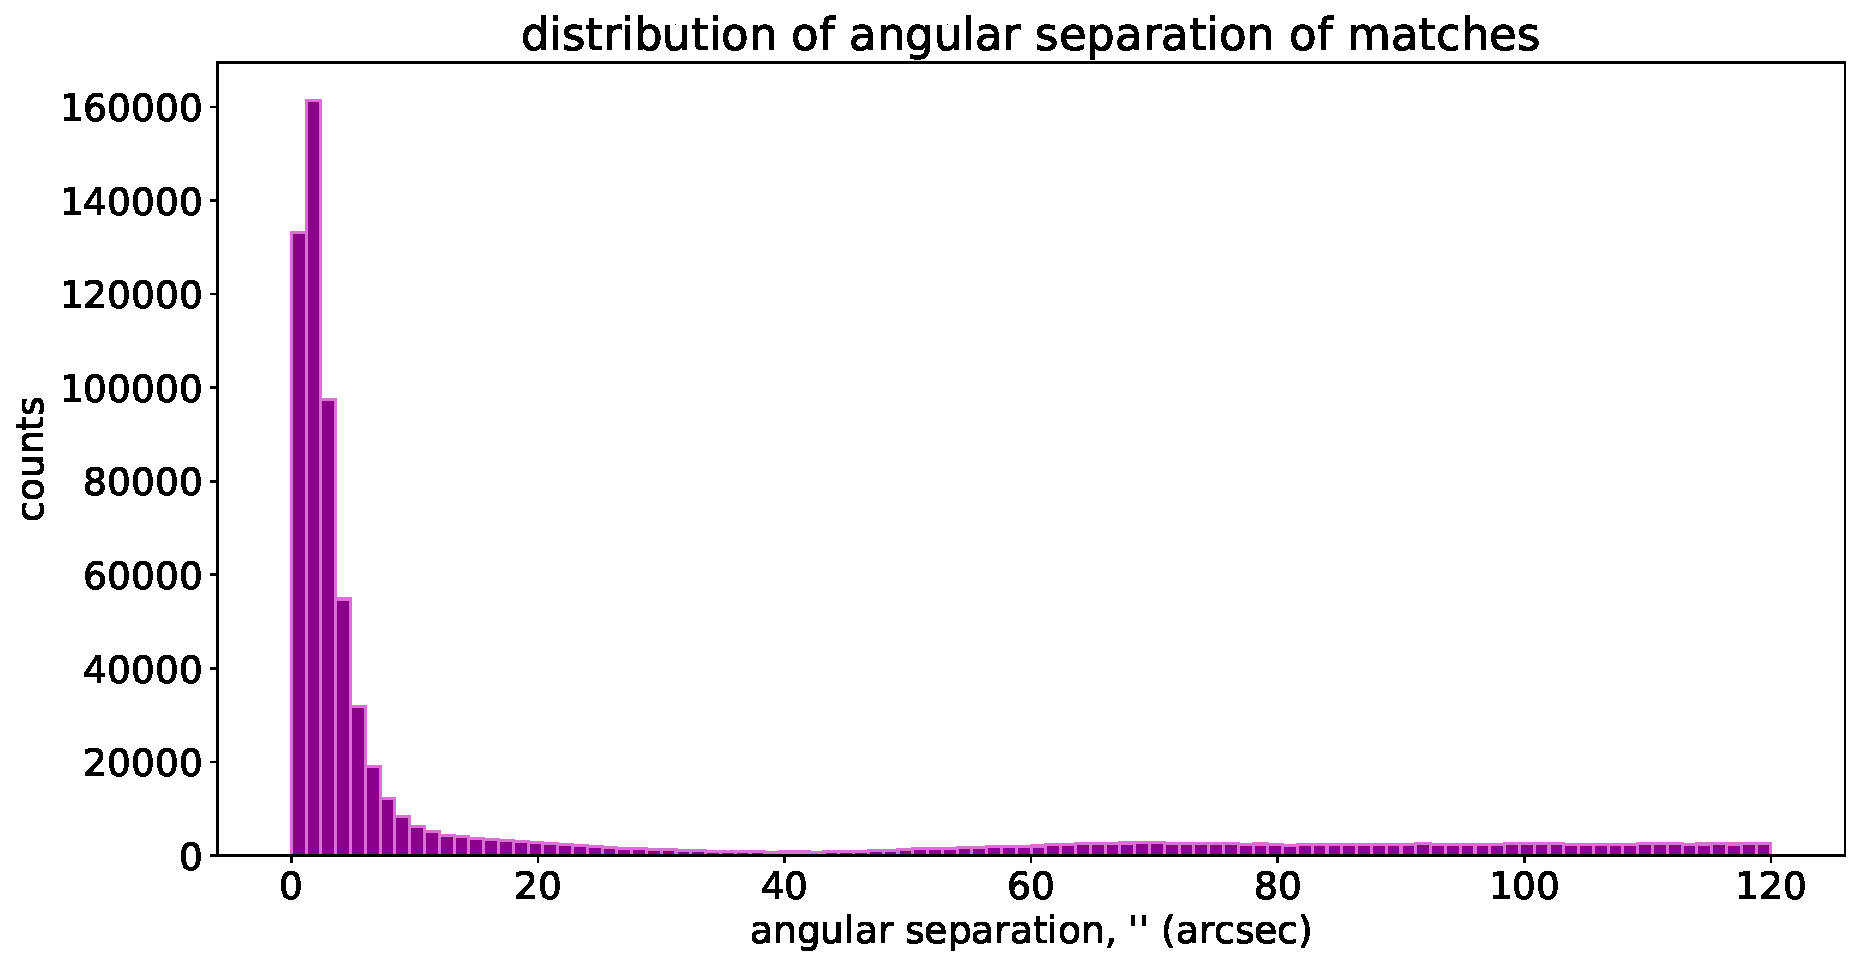
\includegraphics[width=\textwidth]{pics/hist_angle.pdf}
\end{figure}
\end{frame}

\begin{frame}{Spectral index}
\begin{figure}
    \centering
    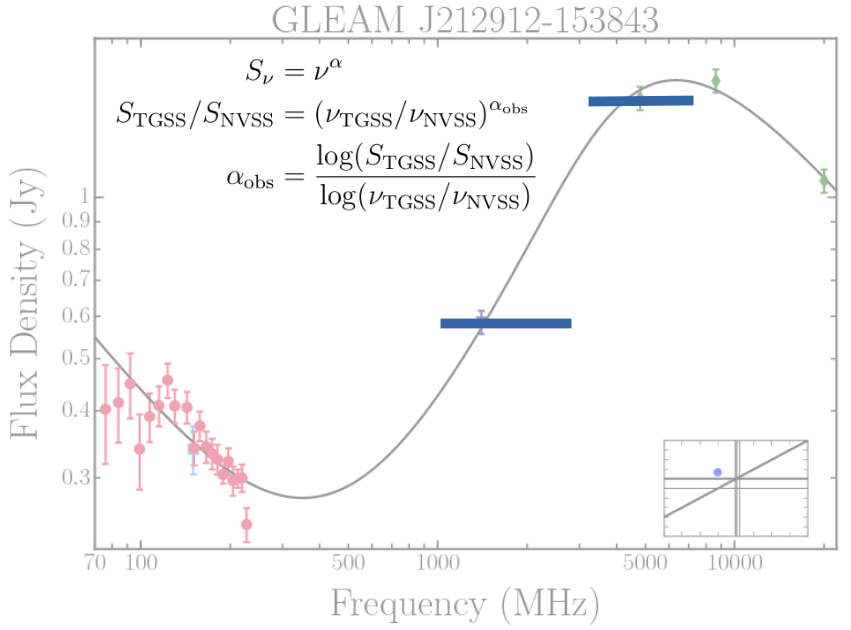
\includegraphics[height=0.8\textheight]{pics/gleam2.png}
\end{figure}
\end{frame}

\begin{frame}{Spectral index comparison}
\begin{figure}
    \centering
    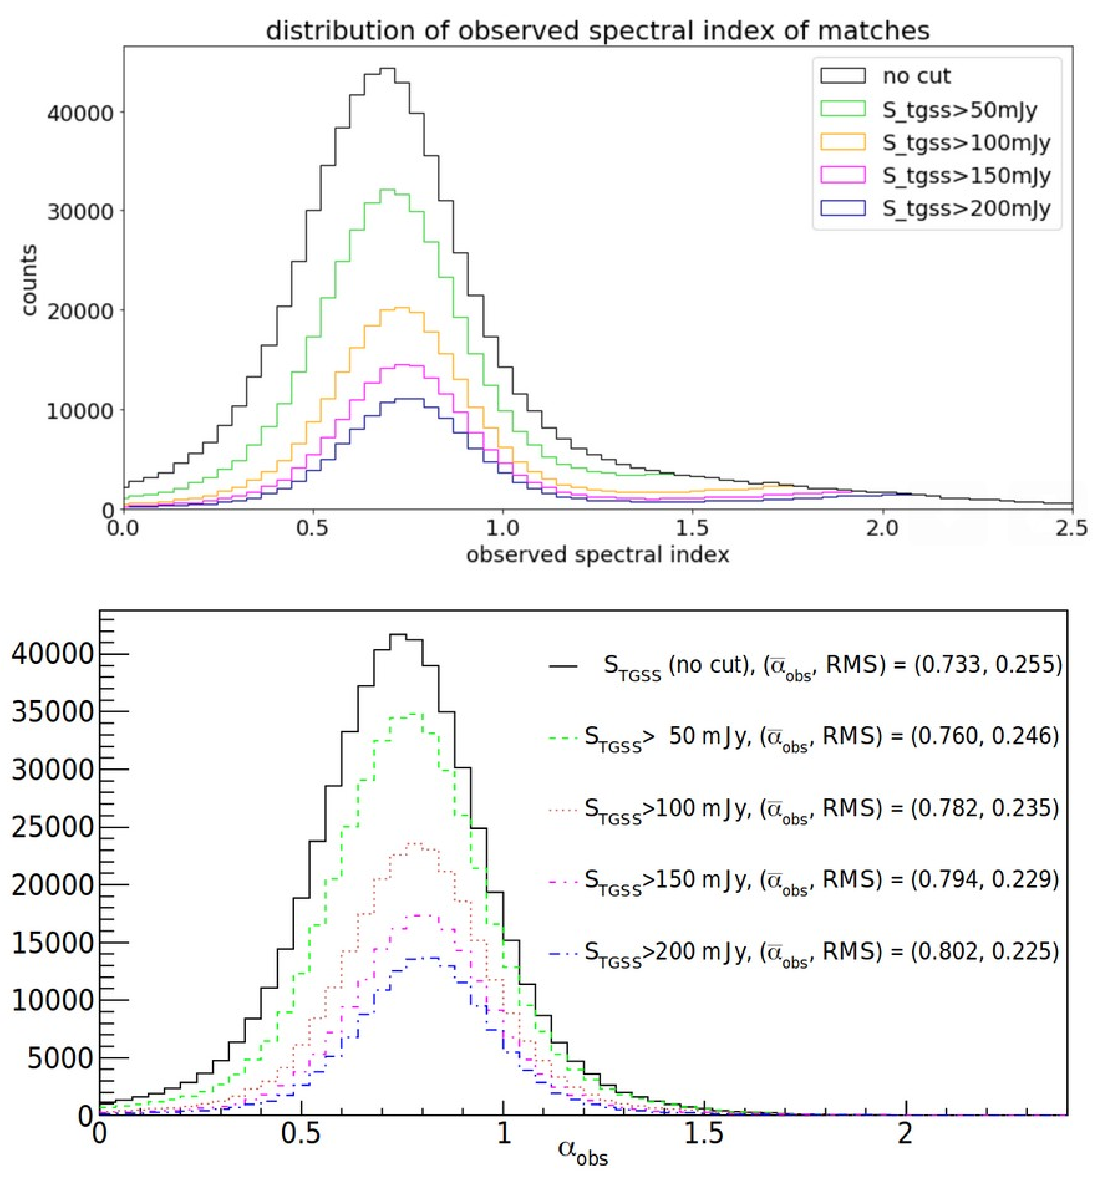
\includegraphics[height=0.78\textheight]{pics/hist_alpha_comparison-cropped.pdf}
    \caption{comparison to Tiwari 2019}
\end{figure}
\end{frame}

\begin{frame}{Supervised machine learning}
\centering
{\Huge
$f: X \longrightarrow Y$
\pause
\begin{center}
Logistic regression
\end{center}
\begin{equation*}
\begin{split}
    f(\vec{x}\,) &= \sigma(\vec{\theta}\cdot\vec{x}+\theta_0) \\
    \sigma(x) &= \frac{1}{1+e^{-x}}
\end{split}
\end{equation*}
}
\end{frame}

\begin{frame}{Binary cross entropy}
\Large{
\begin{equation*}
\begin{split}
    H(y) &= \mathbb{E}_y [- \log_2(y)] \\
    H_f(y) &= \mathbb{E}_y [- \log_2(f)]\\
    &= - (y \log_2(f) + (1-y) \log_2(1-f))
\end{split}
\end{equation*}
}%negative of the log of the likelihood
\end{frame}

\begin{frame}{Logistic regression weights}
\begin{figure}
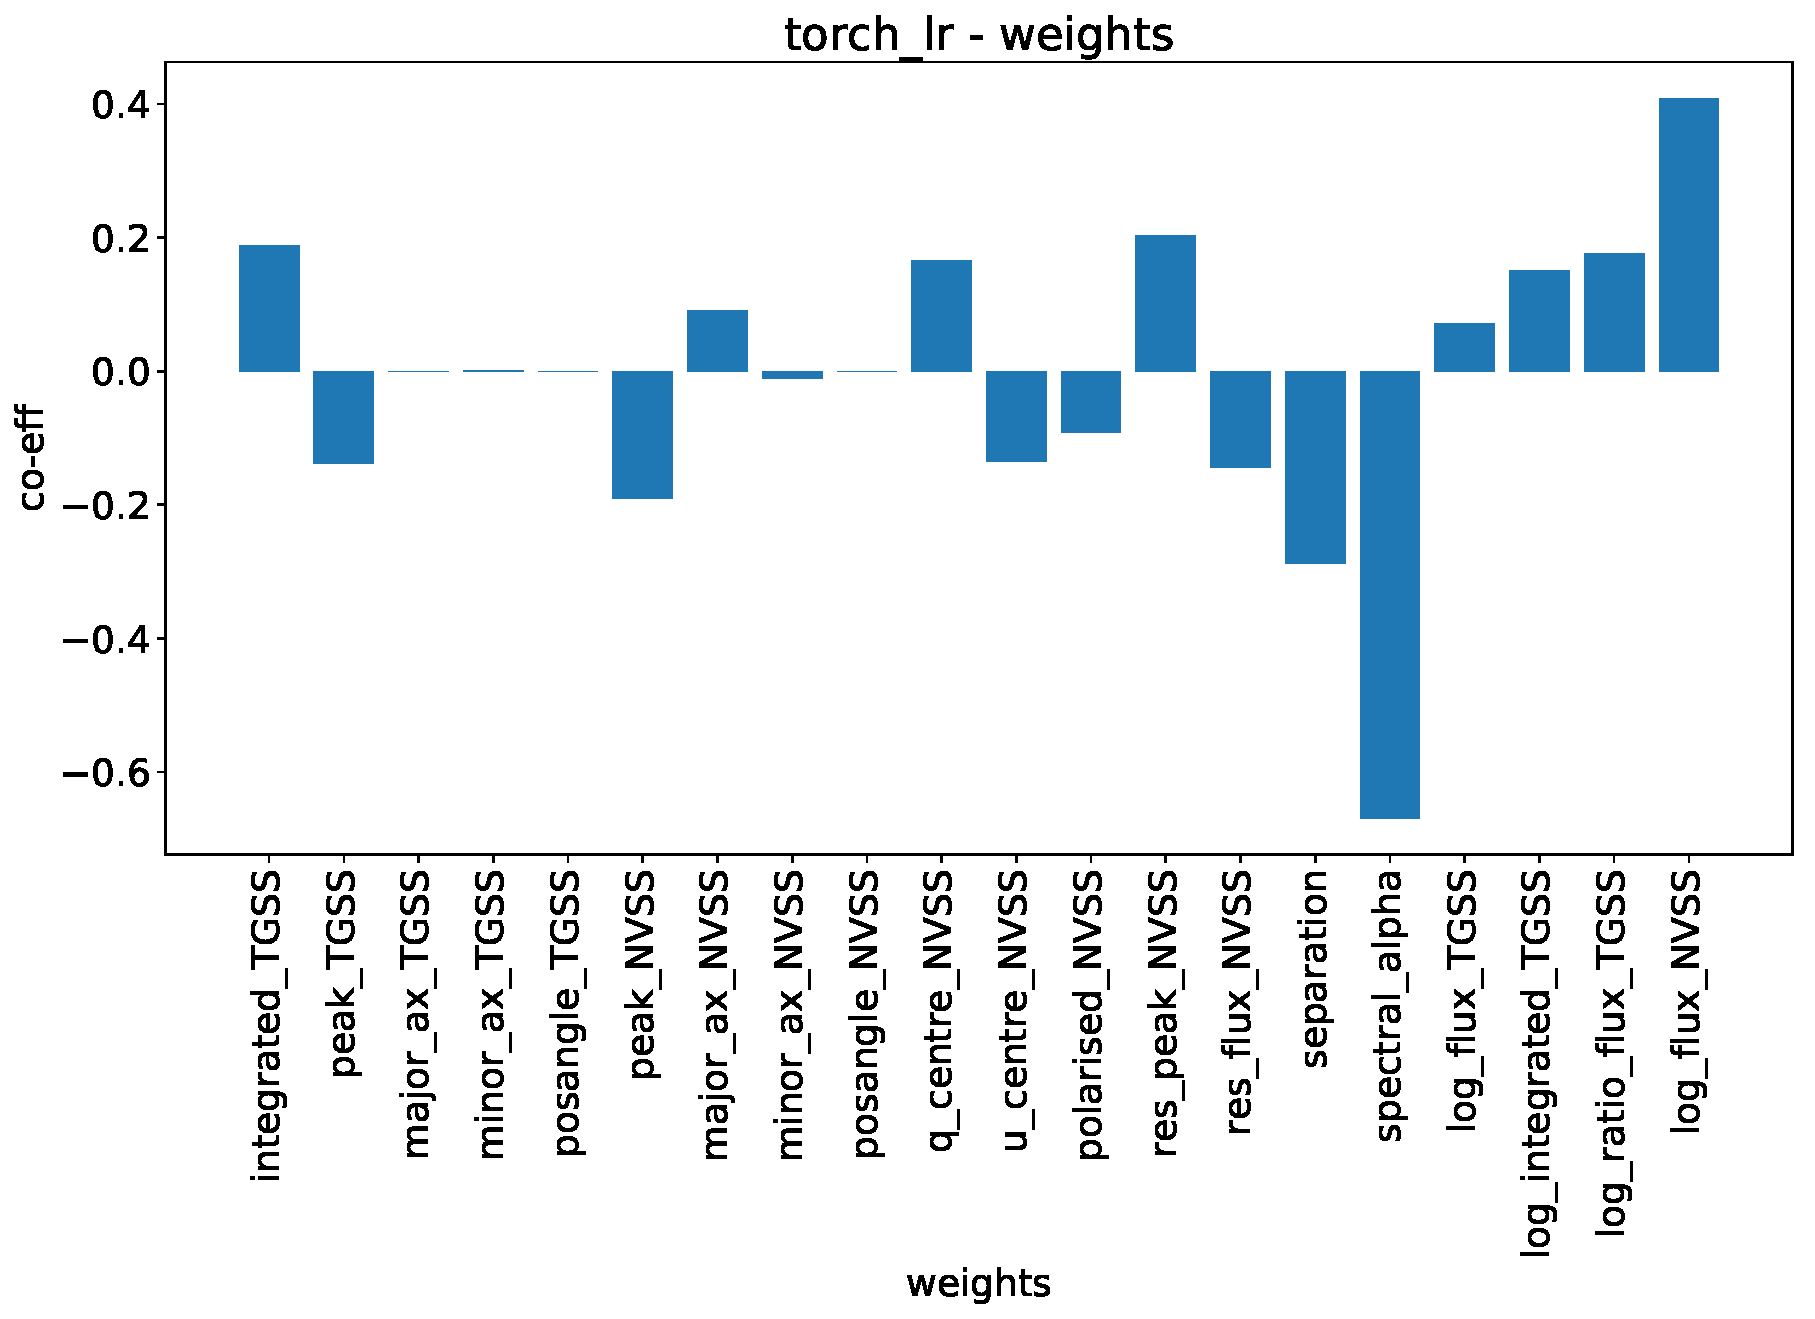
\includegraphics[width=\textwidth]{pics/torch_lr_weights.pdf}
\end{figure}
\end{frame}

\begin{frame}{Logistic regression weights - no separation}
\begin{figure}
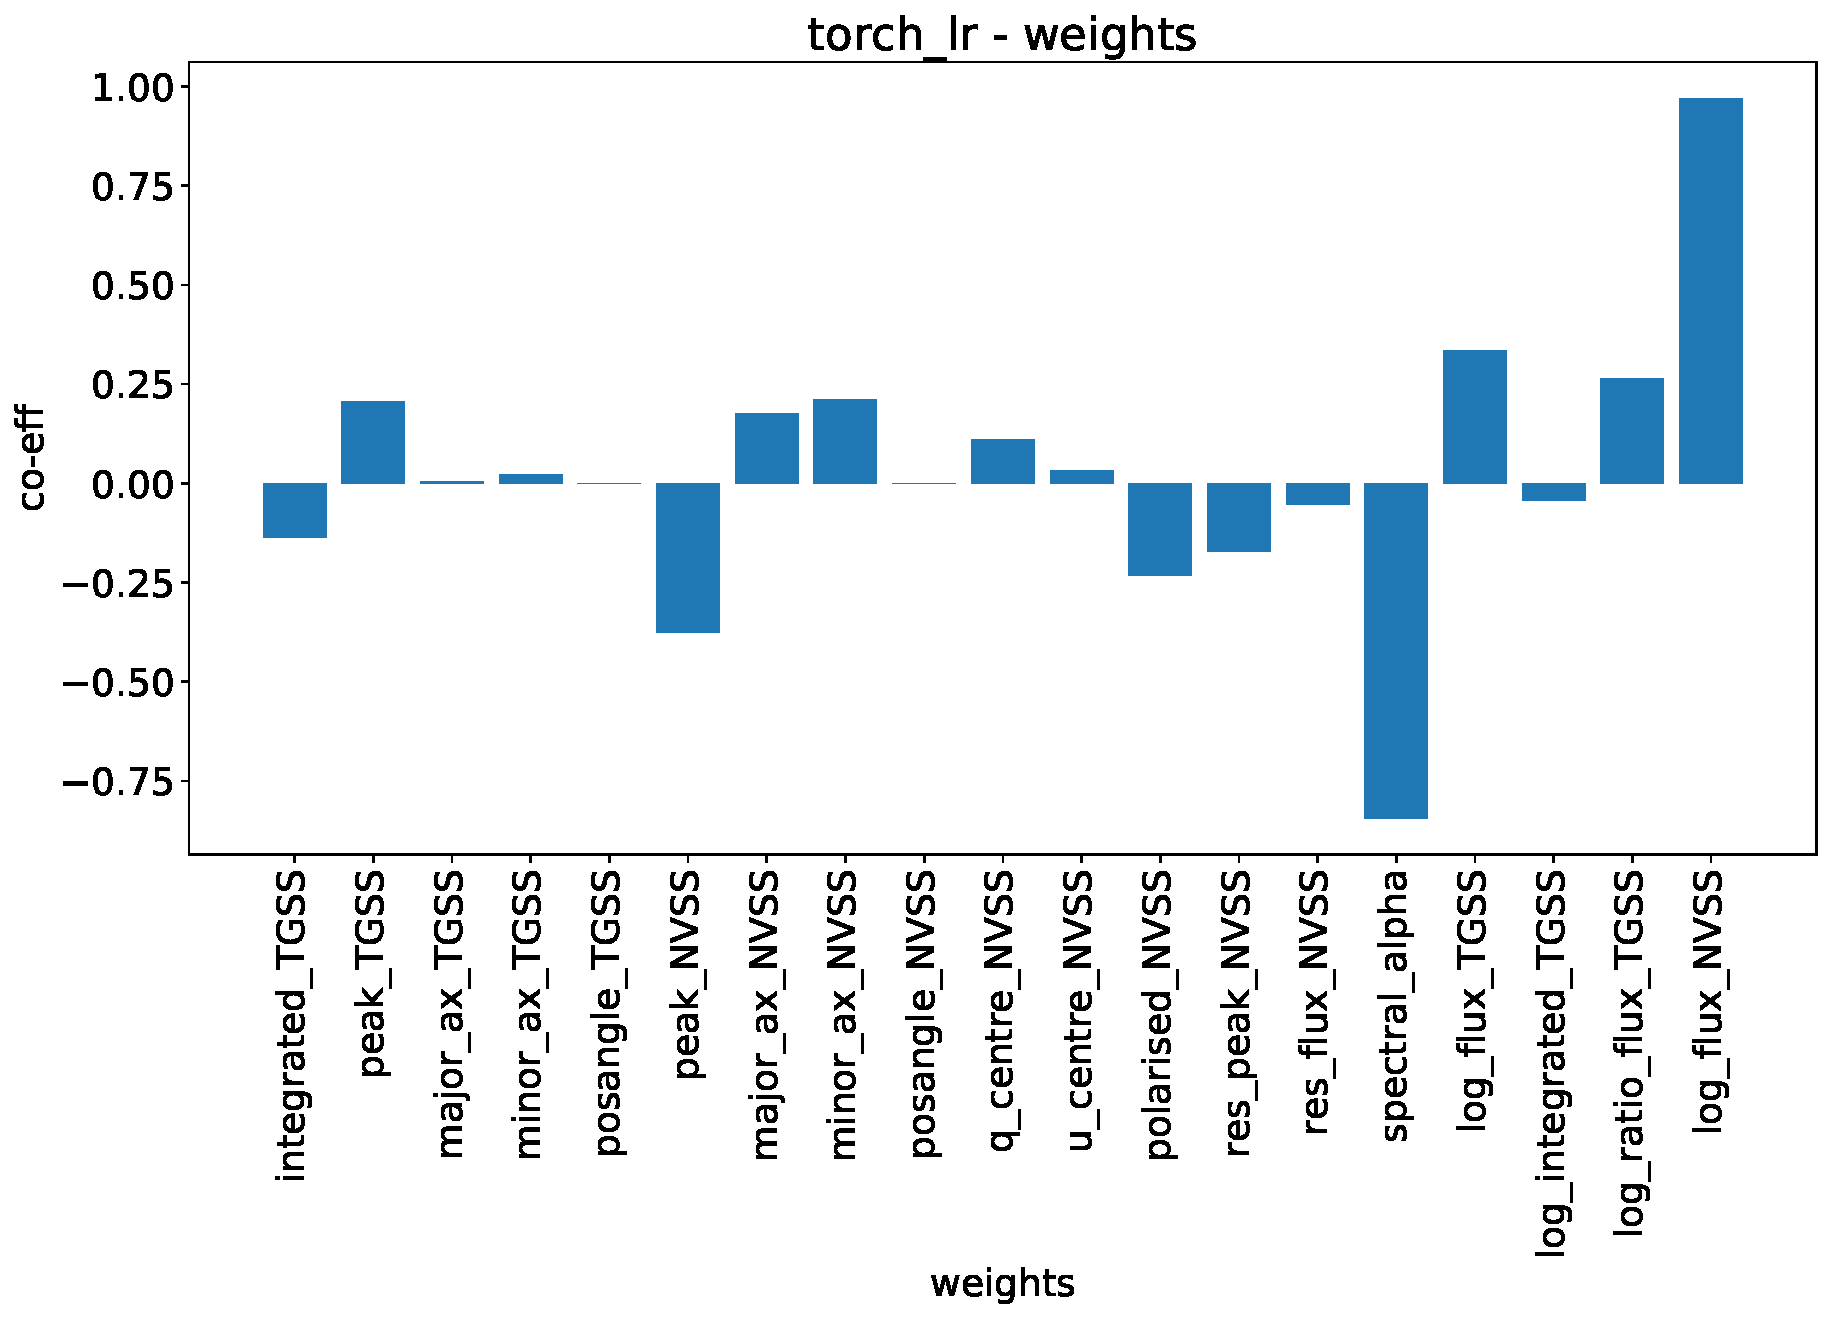
\includegraphics[width=\textwidth]{pics/torch_lr_weights_nosep.pdf}
\end{figure}
\end{frame}

\begin{frame}{Logistic regression predictions}
\begin{figure}
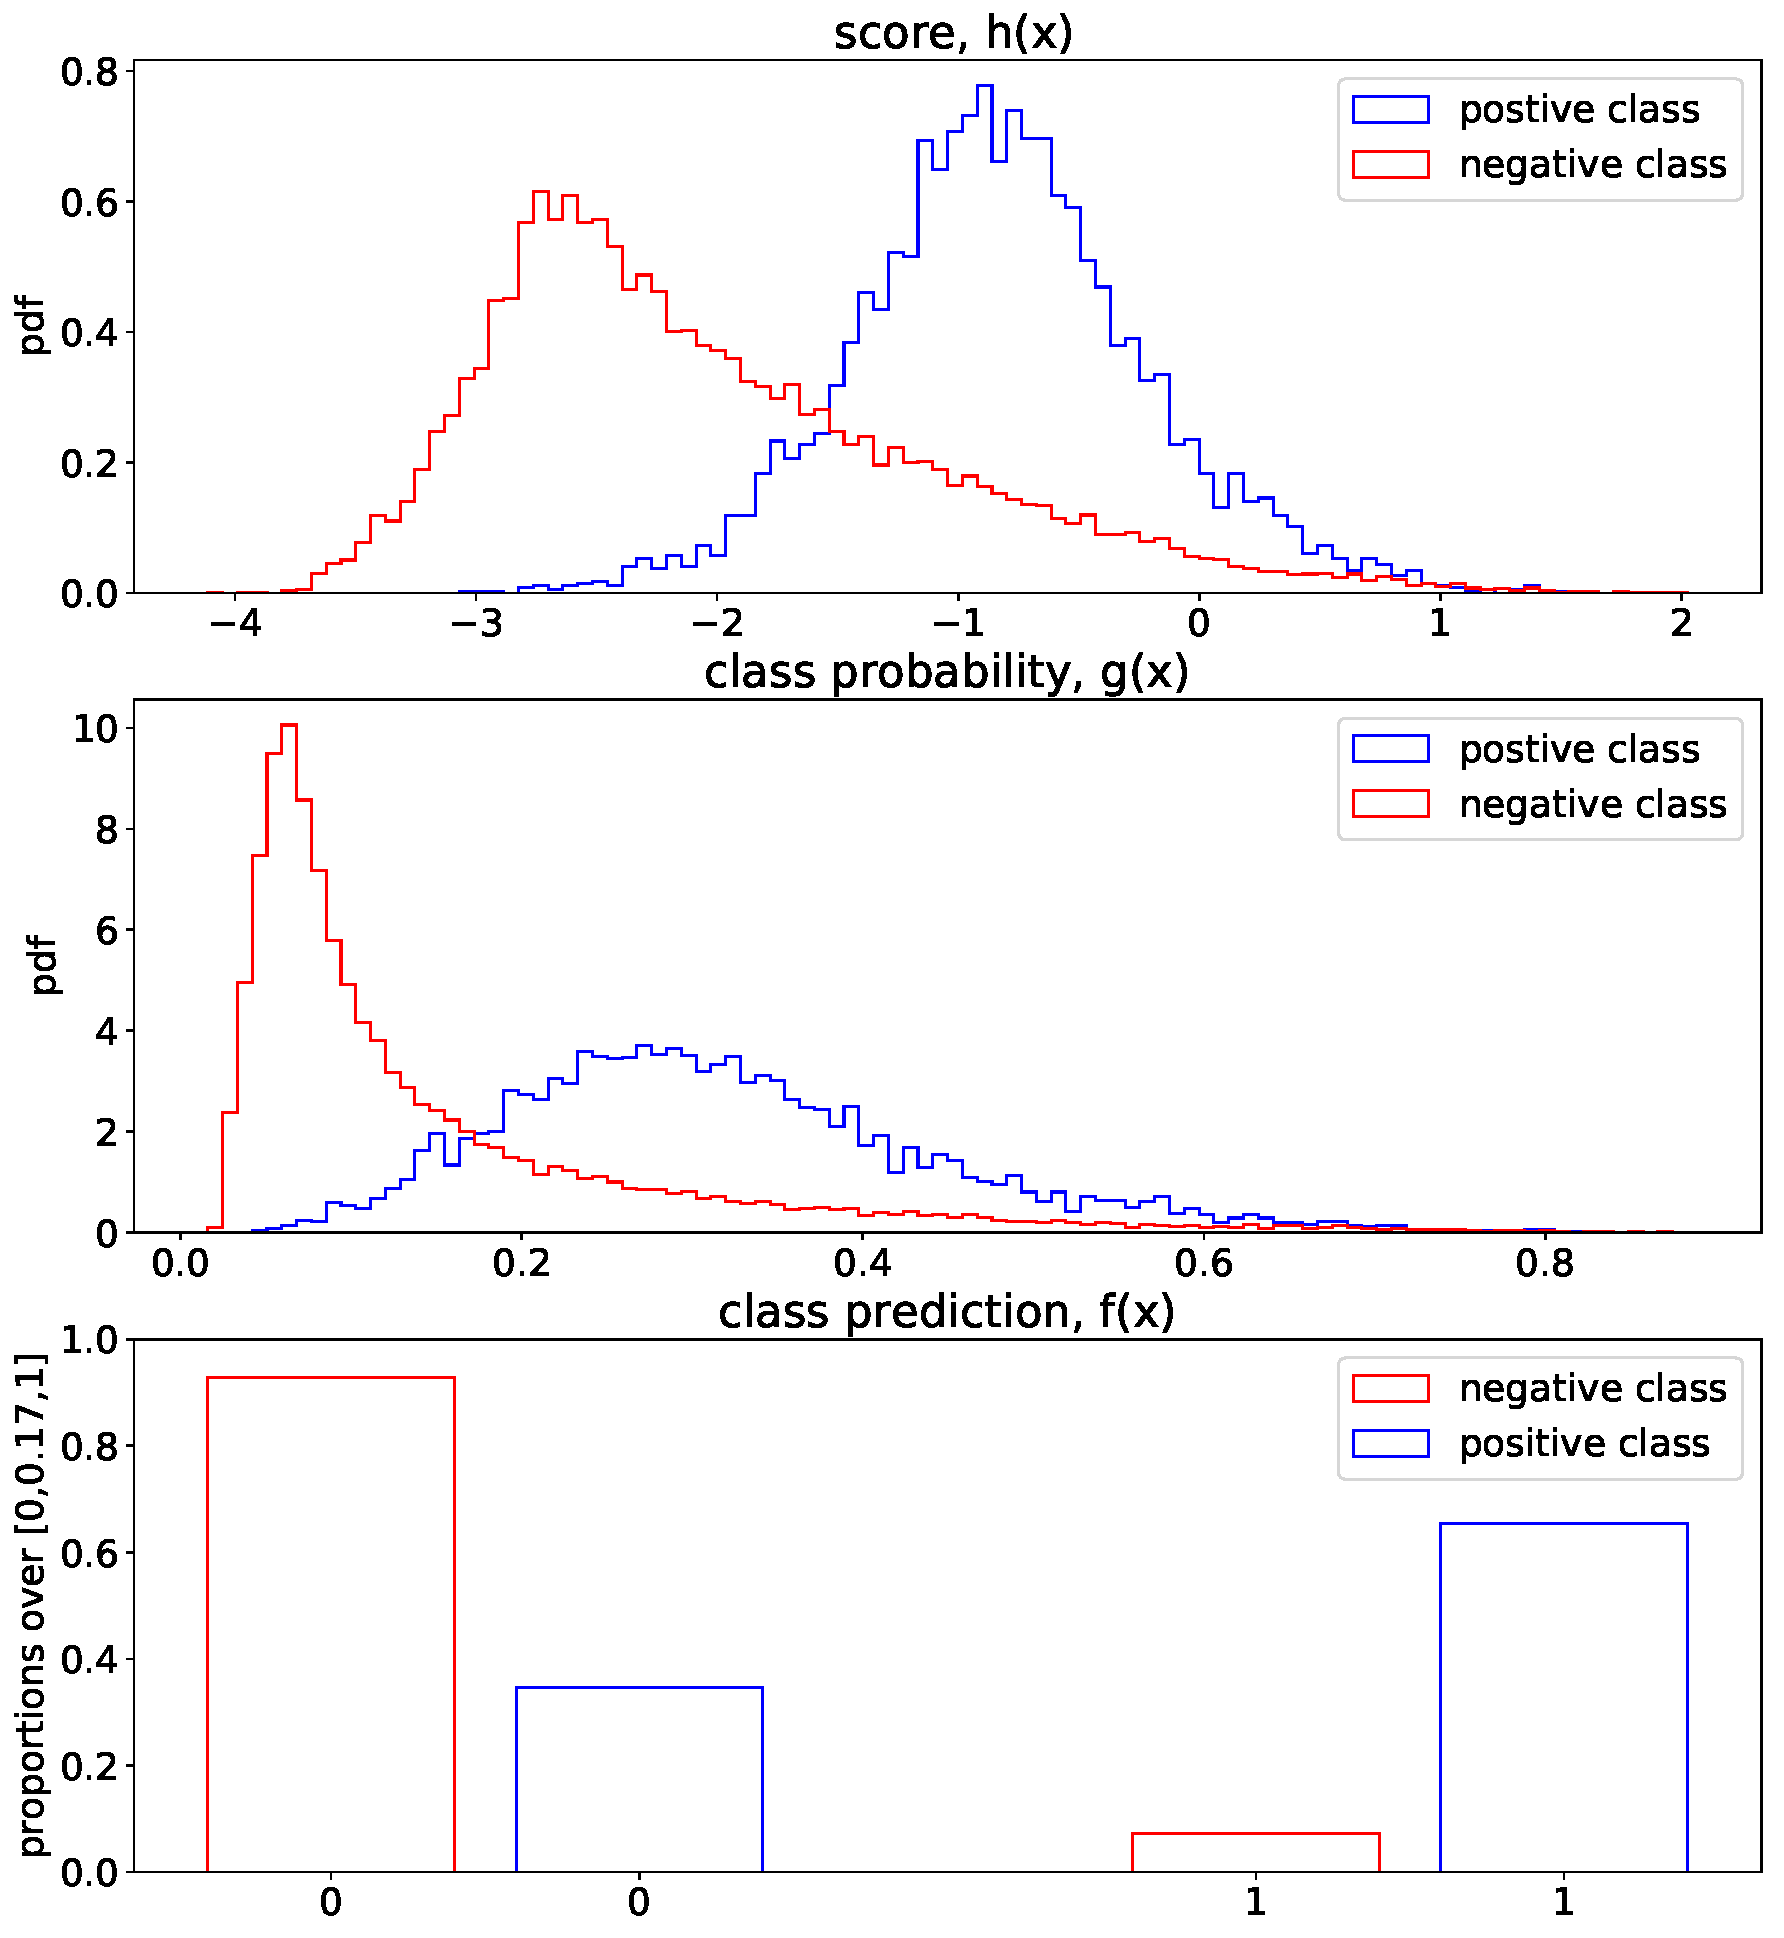
\includegraphics[height=0.85\textheight]{pics/torch_lr_predictions-cropped.pdf}
\end{figure}
\end{frame}

\begin{frame}{Logistic regression accuracy}
\begin{table}[ht]
\centering
\resizebox{\textwidth}{!}{%
\begin{tabular}{rl|c|c|c}
 & & \multicolumn{1}{r|}{accuracy} & \multicolumn{1}{r|}{precision} & \multicolumn{1}{r}{recall} \\ \hline
all features & over patch catalogue & 75.7 & 42.3 & 90.2 \\ \hline
all features & over manual labels & 80 & 80 & 100 \\ \hline
no separation & over patch catalogue & 70.3 & 36.9 & 88.2 \\ \hline
no separation & over manual labels & 80 & 80 & 100
\end{tabular}%
}
\end{table}
\end{frame}

\begin{frame}{Naive transitive partitioning}
\begin{figure}
    \centering
    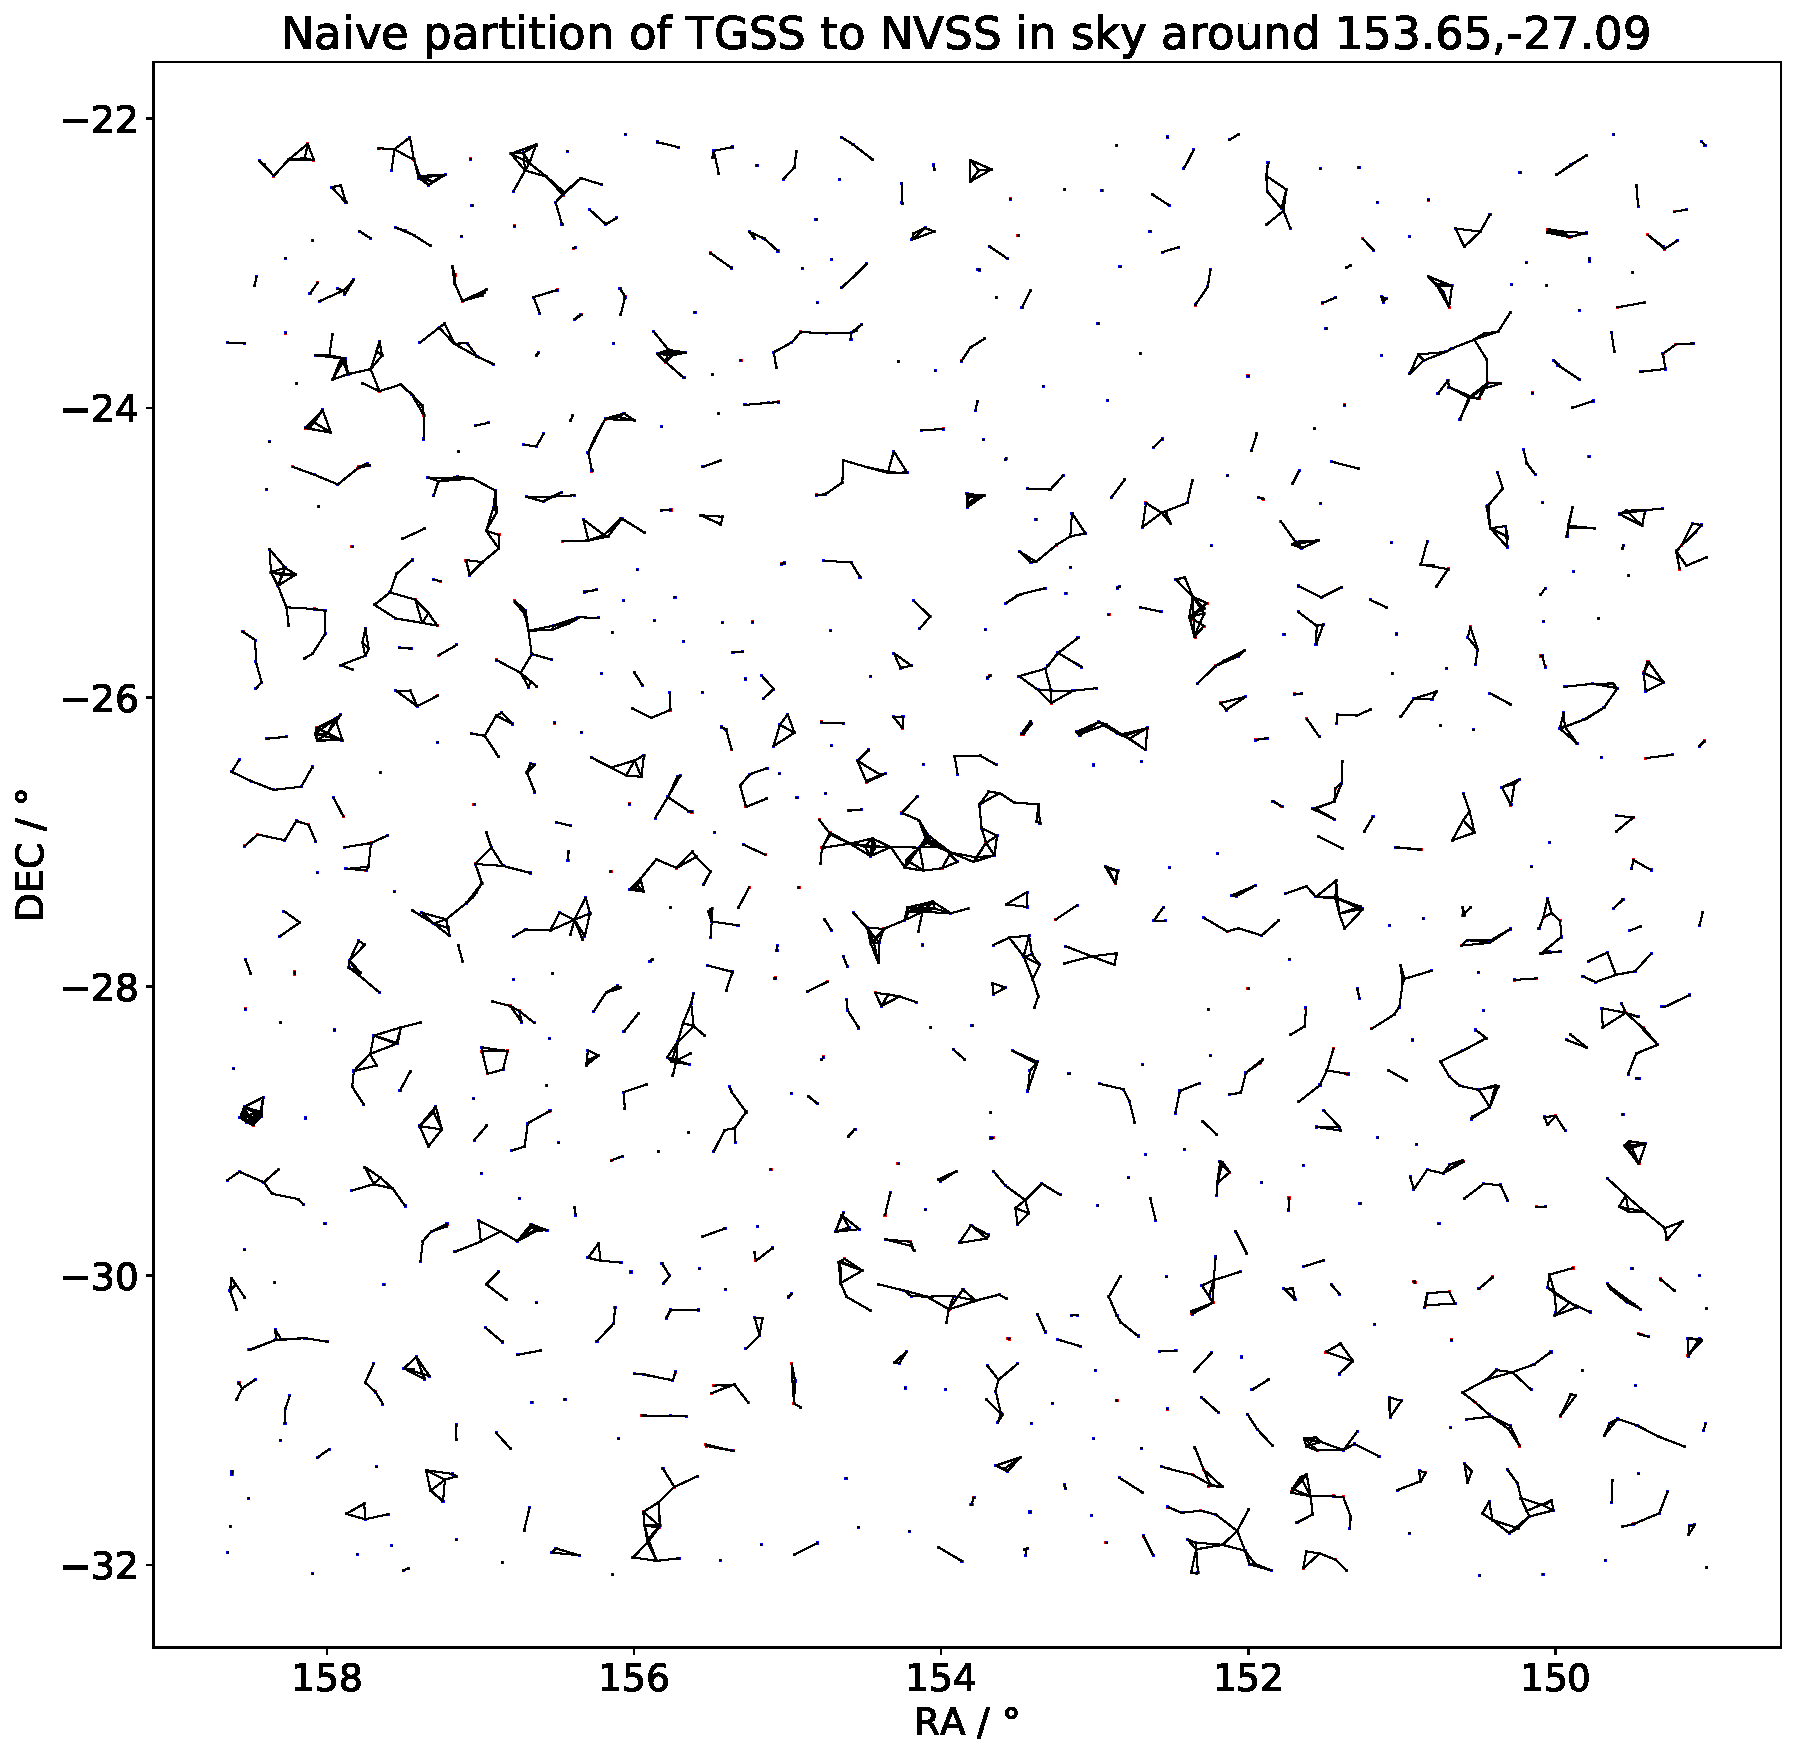
\includegraphics[height=0.85\textheight]{pics/torch_lr_partition.pdf}
\end{figure}
\end{frame}

\begin{frame}{Partition overlay}
\begin{figure}
    \centering
    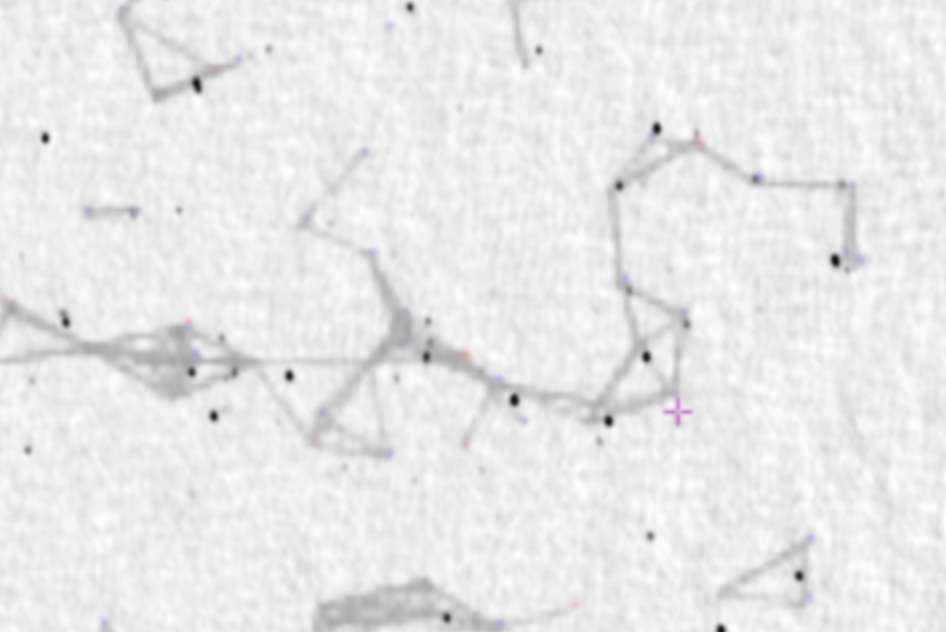
\includegraphics[width=0.95\textwidth]{pics/overlayoverlay.png}
\end{figure}
\end{frame}

\begin{frame}{Conclusions}
\begin{block}{Reproduction of existing results}
% We construct a common catalogue of TGSS to NVSS sources within $\ang{;2;}$ over the shared sky and reproduce the initial results of Tiwari~2019
\end{block}
\begin{exampleblock}{Success of classifier trained on positional matching}
% The classifier does successfully predict the positional matching labels
\end{exampleblock}
\begin{alertblock}{Failure of naive transitive partitioning}
%  Naive transitive partitioning based off a positional matching trained logistic regression classifier does not successfully partition the sky into physical objects
\end{alertblock}
\end{frame}

%%%%%%%% repete primeiro slide %%%%%%%%
\begin{frame}
\titlepage 
\end{frame}

\end{document}
